\section{Introduction}

\begin{frame}{Analogy in CBR}

    \centering\emph{"Every time I forgot my umbrella, it is raining, so if I forgot my umbrella it will rain"}

    \vspace{0.85cm}

    \begin{mdframed}[style=box] 

    A little bit of text
     \end{mdframed}

    \vspace{0.85cm}

    \centering\textbf{Similar situations have similar outcomes}

\end{frame}

%%%%%%%%%%%%%%%%%%%%%%%%%%%%%%%%%%%%%%%%%%%%%%%%%%%%%%%%

\begin{frame}{The CoAT method}
    
    \vspace{0.25cm}

    \begin{mdframed}[style=box] % A simpler example of yellow boxes
         \textbf{Ordinal constraint :} \emph{If $S_0$ is more similar to $S_i$ than to $S_j$ then the same thing should be true for the outcomes}
     \end{mdframed}
    
    \vspace{0.25cm}
    
    \begin{center}
        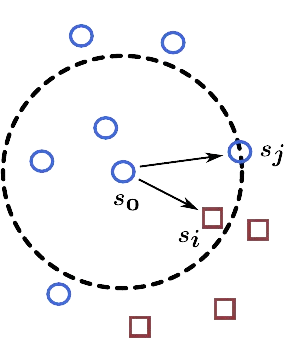
\includegraphics[scale=0.25]{img/logos/pretty.png}
    \end{center}
    
    \vspace{0.25cm}

    \begin{mdframed}[style=box]
         \textbf{The CoAT indicator :} $\Gamma (CB, \sigma_S, \sigma_R)$ = number of triples \\$(S_0, S_i, S_j)$ where the constraint is not respected
     \end{mdframed}
    
\end{frame}

%%%%%%%%%%%%%%%%%%%%%%%%%%%%%%%%%%%%%%%%%%%%%%%%%%%%%%%%

\begin{frame}<1>[label=dist]{Distance} % you will see what dark magic i will do with that label

    \vspace{0.5cm} % some math examples
    
    \textbf{Euclidean Distance:} $$d_E = \sqrt{(x_1 - x_2)^2+(y_1 - y_2)^2}$$

    \textbf{Manhattan Distance:} $$ d_{Man} = |x_1-x_2|+|y_1-y_2|$$

    \textbf{The Minkoswki Distance:} $$d_{Mk}^p =  [(x_1-x_2)^p + (y_1-y_2)^p]^{\frac{1}{p}} $$

    \textbf{Mahalanobis Distance:} $$D_{\text{mahal}}= \sqrt{(x-y)^T M^{-1} (x-y)}$$
    
\end{frame}

%%%%%%%%%%%%%%%%%%%%%%%%%%%%%%%%%%%%%%%%%%%%%%%%%%%%%%%%

\section{Regression}
\subsection{With Generated Data}

\begin{frame}{With Generated Data (1)}
    Generating Function : $2 \times x + 1$
    
    Noise function : \textit{Gaussian distribution with $\sigma$ = 100 and $\mu$ = 0}
    \begin{figure}
        \centering
        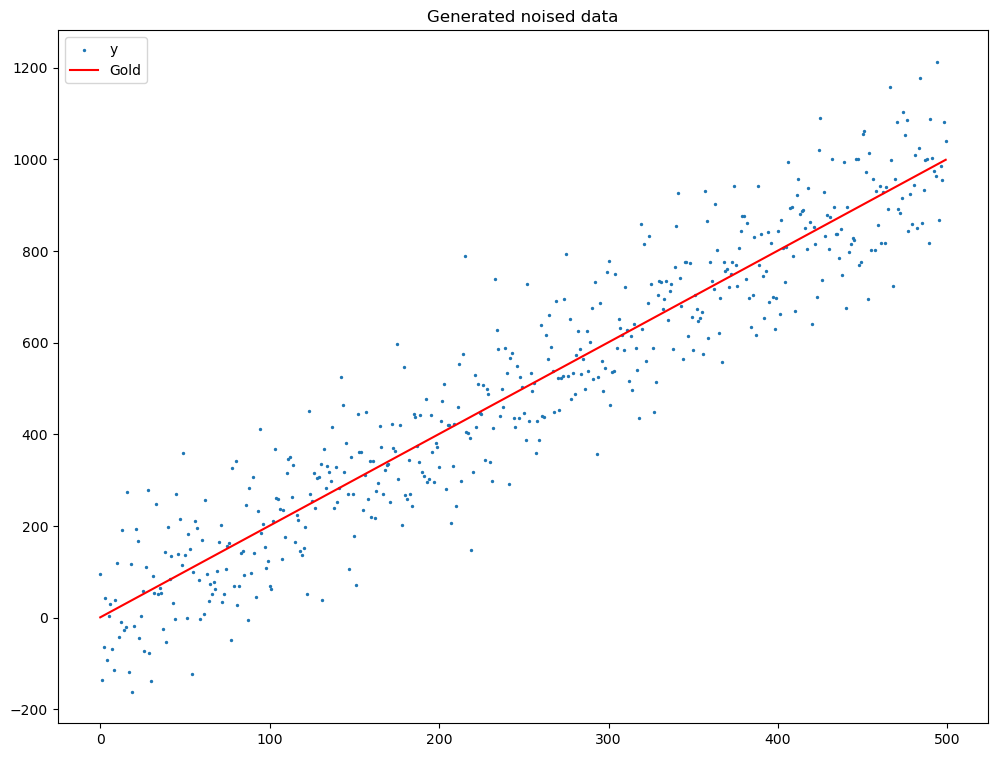
\includegraphics[scale=0.35]{img/a.png}
    \end{figure}
\end{frame}

%%%%%%%%%%%%%%%%%%%%%%%%%%%%%%%%%%%%%%%%%%%%%%%%%%%%%%%%

\begin{frame}<1>[label=zooms]{With Generated Data (2)}

    \framezoom<1><2>(0cm,0cm)(4cm,3.7cm) % we specify where to zoom (coordinate of the top-left 
    \framezoom<1><3>(6cm,0cm)(4cm,3.7cm) % angle of the rectangle)(size rectangle)
	
    \begin{columns} % A better way to have 2 columns than minipage, doesn't work in the yellow boxes
        \begin{column}{0.48\textwidth}
            \begin{figure}
                \centering
                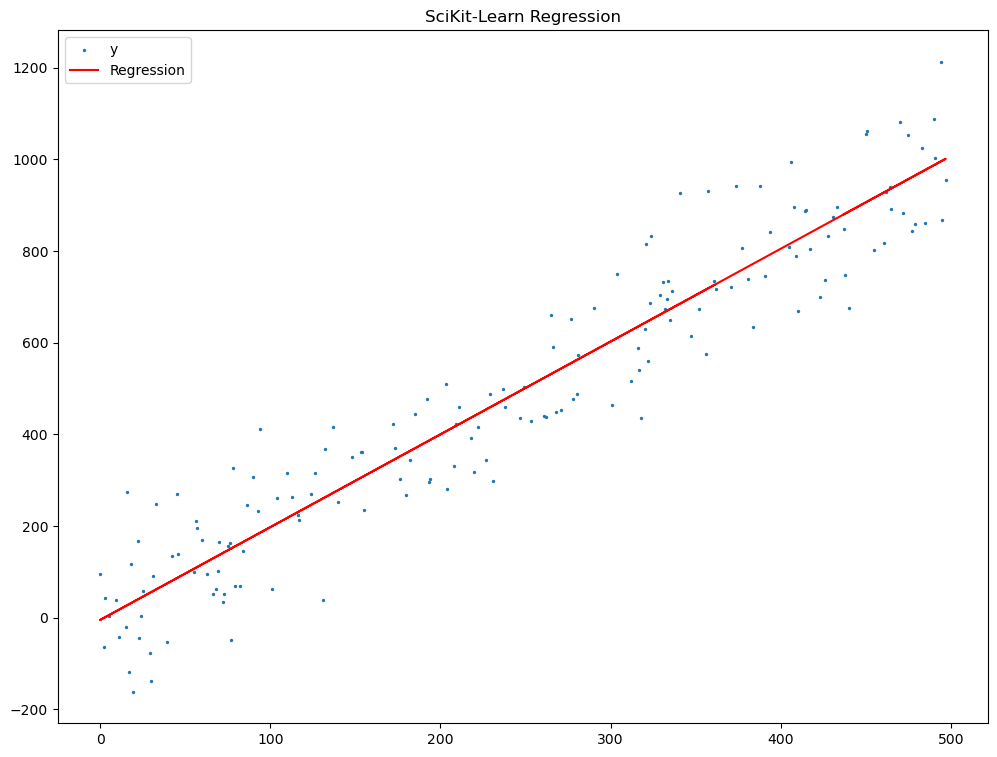
\includegraphics[width=0.9\textwidth]{img/b.png}
                Regression with SciKit-learn
            \end{figure}
        \end{column}
        \begin{column}{0.48\textwidth}
            \begin{figure}
                \centering
                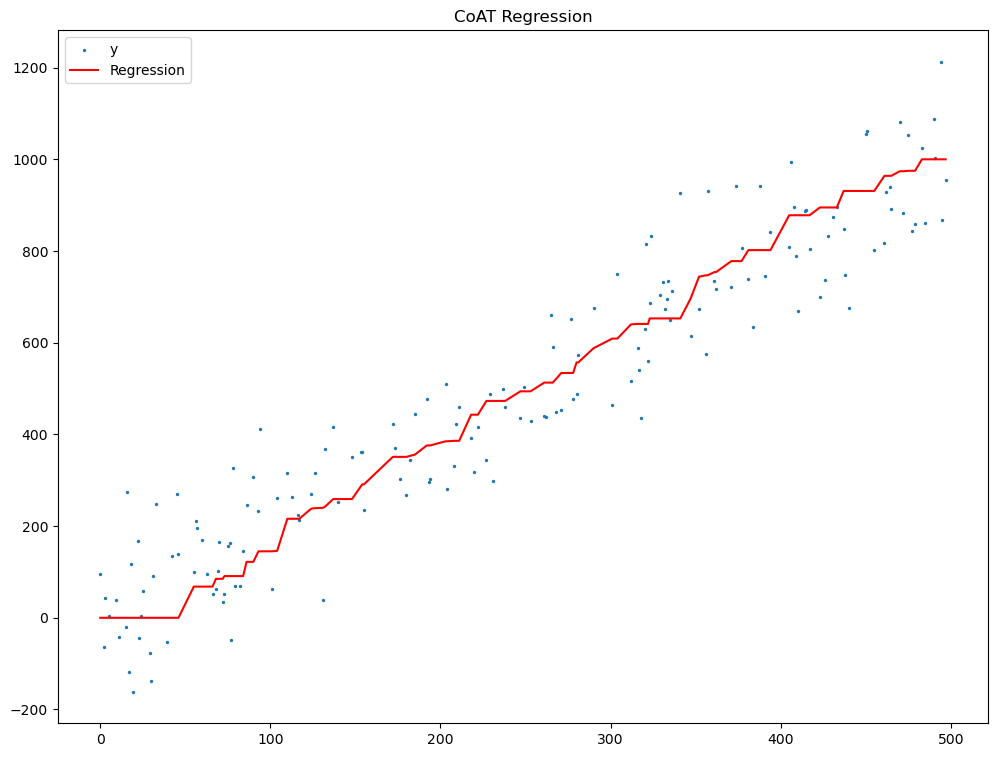
\includegraphics[width=0.9\textwidth]{img/c.png}
                Regression with CoAT
            \end{figure}
        \end{column}
    \end{columns}

    \vspace{0.3cm}

    \begin{mdframed}[style=box]
    \begin{itemize}
        \item Impact of different source and outcomes similarities
        \item Comparison with NN for benchmarking
        \item Real Datasets (multidimensions)
    \end{itemize}
     \end{mdframed}
    
\end{frame}

\againframe<2->[plain]{zooms} % to have it without title

%%%%%%%%%%%%%%%%%%%%%%%%%%%%%%%%%%%%%%%%%%%%%%%%%%%%%%%%

\againframe<2>{dist} % dark magic, i put an old frame again

%%%%%%%%%%%%%%%%%%%%%%%%%%%%%%%%%%%%%%%%%%%%%%%%%%%%%%%%

\begin{frame}{Where do we live ?}

    \begin{tikzpicture}[
    spy using outlines={
      circle,
      magnification=10,
      size=5cm,
      connect spies}]
    \node[inner sep=0pt] {\pgfimage[width=0.4\textwidth]{img/map.jpg}};
    \only<2>{\spy[red!70!black] on (1.2,0.8) in node at (.5\textwidth,0);}
    \end{tikzpicture} % on (0,0) -> center of the picture, (pos, pos) -> top-right corner
    % (neg, neg) -> bottom-left corner
    \only<3>{
        \raisebox{9ex}{
            \begin{minipage}{0.5\textwidth} % The raisebox in minipage technique again
            \centering \Large Elle est pas belle ma France ?
            \end{minipage}
        }}
    
\end{frame}

%%%%%%%%%%%%%%%%%%%%%%%%%%%%%%%%%%%%%%%%%%%%%%%%%%%%%%%%

\subsection{Problems}

\begin{frame}{The problem(s) with regression}
    \textbf{Why I have lost my mind:} A prediction issue

    \begin{itemize}
        \item 10+mn for 165 cases
        \vspace{0.2cm}
        \item Prediction item by item vs prediction by list
        \vspace{0.2cm}
        \item A problem with $y\_values$ ?
        \begin{itemize}
            \item \textit{range(function(500))}
            \item \textit{range(0,function(500),10)}
            \item \textit{range(0,function(500),100)}
        \end{itemize}
        \vspace{0.2cm}
        \item A problem with the number of case ?


    \end{itemize}
    
\end{frame}
